%% bare_conf.tex
%% V1.3
%% 2007/01/11
%% by Michael Shell
%% See:
%% http://www.michaelshell.org/
%% for current contact information.
%%
%% This is a skeleton file demonstrating the use of IEEEtran.cls
%% (requires IEEEtran.cls version 1.7 or later) with an IEEE conference paper.
%%
%% Support sites:
%% http://www.michaelshell.org/tex/ieeetran/
%% http://www.ctan.org/tex-archive/macros/latex/contrib/IEEEtran/
%% and
%% http://www.ieee.org/

%%*************************************************************************
%% Legal Notice:
%% This code is offered as-is without any warranty either expressed or
%% implied; without even the implied warranty of MERCHANTABILITY or
%% FITNESS FOR A PARTICULAR PURPOSE!
%% User assumes all risk.
%% In no event shall IEEE or any contributor to this code be liable for
%% any damages or losses, including, but not limited to, incidental,
%% consequential, or any other damages, resulting from the use or misuse
%% of any information contained here.
%%
%% All comments are the opinions of their respective authors and are not
%% necessarily endorsed by the IEEE.
%%
%% This work is distributed under the LaTeX Project Public License (LPPL)
%% ( http://www.latex-project.org/ ) version 1.3, and may be freely used,
%% distributed and modified. A copy of the LPPL, version 1.3, is included
%% in the base LaTeX documentation of all distributions of LaTeX released
%% 2003/12/01 or later.
%% Retain all contribution notices and credits.
%% ** Modified files should be clearly indicated as such, including  **
%% ** renaming them and changing author support contact information. **
%%
%% File list of work: IEEEtran.cls, IEEEtran_HOWTO.pdf, bare_adv.tex,
%%                    bare_conf.tex, bare_jrnl.tex, bare_jrnl_compsoc.tex
%%*************************************************************************

% *** Authors should verify (and, if needed, correct) their LaTeX system  ***
% *** with the testflow diagnostic prior to trusting their LaTeX platform ***
% *** with production work. IEEE's font choices can trigger bugs that do  ***
% *** not appear when using other class files.                            ***
% The testflow support page is at:
% http://www.michaelshell.org/tex/testflow/



% Note that the a4paper option is mainly intended so that authors in
% countries using A4 can easily print to A4 and see how their papers will
% look in print - the typesetting of the document will not typically be
% affected with changes in paper size (but the bottom and side margins will).
% Use the testflow package mentioned above to verify correct handling of
% both paper sizes by the user's LaTeX system.
%
% Also note that the "draftcls" or "draftclsnofoot", not "draft", option
% should be used if it is desired that the figures are to be displayed in
% draft mode.
%
%\documentclass[conference]{IEEEtran}
\documentclass[conference,a4paper]{IEEEtran}
% Add the compsoc option for Computer Society conferences.
%
% If IEEEtran.cls has not been installed into the LaTeX system files,
% manually specify the path to it like:
% \documentclass[conference]{../sty/IEEEtran}





% Some very useful LaTeX packages include:
% (uncomment the ones you want to load)


% *** MISC UTILITY PACKAGES ***
\usepackage[cmex10]{amsmath}
\usepackage{xcolor}
\usepackage{siunitx}
\sisetup{range-phrase=--}
\DeclareSIUnit\year{yr}
\usepackage{booktabs}
\usepackage{float}
\usepackage{newtxtext,newtxmath}
% \usepackage{geometry} % just not to bother with the table width
\usepackage{graphicx}
% \usepackage{filecontents}
\usepackage{tabularx,colortbl}
\usepackage{booktabs}
\usepackage{pgfplots}
\usepackage{standalone}
\usepackage{tikz}
\tikzset{
font={\fontsize{8pt}{8}\selectfont}}
\usepackage{tikzscale} % Scale the figure not the font
\pgfplotsset{compat=newest}
\usepackage{physics}
\usepackage{chemfig}
\usepackage[version=3]{mhchem}

% *** CITATION PACKAGES ***
%
%\usepackage{cite}
% cite.sty was written by Donald Arseneau
% V1.6 and later of IEEEtran pre-defines the format of the cite.sty package
% \cite{} output to follow that of IEEE. Loading the cite package will
% result in citation numbers being automatically sorted and properly
% "compressed/ranged". e.g., [1], [9], [2], [7], [5], [6] without using
% cite.sty will become [1], [2], [5]--[7], [9] using cite.sty. cite.sty's
% \cite will automatically add leading space, if needed. Use cite.sty's
% noadjust option (cite.sty V3.8 and later) if you want to turn this off.
% cite.sty is already installed on most LaTeX systems. Be sure and use
% version 4.0 (2003-05-27) and later if using hyperref.sty. cite.sty does
% not currently provide for hyperlinked citations.
% The latest version can be obtained at:
% http://www.ctan.org/tex-archive/macros/latex/contrib/cite/
% The documentation is contained in the cite.sty file itself.


% correct bad hyphenation here
\hyphenation{op-tical net-works semi-conduc-tor}

\DeclareRobustCommand*{\IEEEauthorrefmark}[1]{\raisebox{0pt}[0pt][0pt]{\textsuperscript{\footnotesize #1}}}

\begin{document}
%
% paper title
% can use linebreaks \\ within to get better formatting as desired
\title{Remote Monitoring of Absorbable Cardiovascular Stents using mm-waves}



% author names and affiliations
% use a single column layout for the different affiliations.
% In case the affiliation is too long then use \\ to create multiple lines, as shown in affiliation 4
% Too long lines can result in margin upload warnings ....
\author{\IEEEauthorblockN{
Hasan Abbas\IEEEauthorrefmark{1},   % 1st author, 1st affiliations
Qammer Abbasi\IEEEauthorrefmark{2},   % 2nd author, 2nd affiliations
Younes Boudjemline\IEEEauthorrefmark{3},    % 3rd author, 3rd affiliations
Ziyad Hijazi\IEEEauthorrefmark{3},
Bilal Mansoor\IEEEauthorrefmark{4},
Khalid Qaraqe\IEEEauthorrefmark{1}      % 4th author, 4th affiliations
}                                     % ...
%\\
\IEEEauthorblockA{\IEEEauthorrefmark{1}% 1st affiliations
Department of ECEN, Texas A\&M University at Qatar}
\IEEEauthorblockA{\IEEEauthorrefmark{2}% 2nd affiliations
School of Engineering, University of Glasgow}
\IEEEauthorblockA{\IEEEauthorrefmark{3}% 3rd affiliations
Department of Pediatric Cardiology, Sidra Medicine}
\IEEEauthorblockA{\IEEEauthorrefmark{4}% 4th affiliations
Department of MEEN, Texas A\&M University at Qatar,
}
\IEEEauthorblockA{ \emph{hasan.abbas@qatar.tamu.edu} }
}

% conference papers do not typically use \thanks and this command
% is locked out in conference mode. If really needed, such as for
% the acknowledgment of grants, issue a \IEEEoverridecommandlockouts
% after \documentclass



% use for special paper notices
%\IEEEspecialpapernotice{(Invited Paper)}




% make the title area
\maketitle


\begin{abstract}
  %\boldmath
  In this paper, we propose a corrosion monitoring scheme for the absorbable cardiovascular stents composed of magnesium alloys. We show that the structural integrity of such mesh-type tubular stents can be evaluated using millimeter-scale electromagnetic waves. With the passage of time, the strut thickness of the stent decreases due to corrosion which is subsequently observed in terms of a frequency shift in the simulated scattering response.
\end{abstract}
% IEEEtran.cls defaults to using nonbold math in the Abstract.
% This preserves the distinction between vectors and scalars. However,
% if the conference you are submitting to favors bold math in the abstract,
% then you can use LaTeX's standard command \boldmath at the very start
% of the abstract to achieve this. Many IEEE journals/conferences frown on
% math in the abstract anyway.

% no keywords
%{\smallskip \keywords antenna, propagation, measurement.}
% Keywords
\textbf{\small{\emph{biodegradable cardiovascular stents, non-destructive evaluation, millimeter waves}}}


% For peer review papers, you can put extra information on the cover
% page as needed:
% \ifCLASSOPTIONpeerreview
% \begin{center} \bfseries EDICS Category: 3-BBND \end{center}
% \fi
%
% For peerreview papers, this IEEEtran command inserts a page break and
% creates the second title. It will be ignored for other modes.
\IEEEpeerreviewmaketitle

\vspace{7pt}
\section{Introduction}
% no \IEEEPARstart
Cardiovascular disease (CVD) is the leading cause of death worldwide, and it accounted for an estimated 30\% of all deaths in the year 2013 globally \cite{benjamin_heart_2017}. Clogging of the heart vessels is the biggest factor responsible for the development of the CVD. These days, it is a common clinical practice to reopen the heart vessels through balloon angioplasty, and place a mesh-type metallic scaffolding tube called a stent to reinforce the vessel walls.  However, due to the long-standing presence of a metallic foreign object in the form of a stent, serious health complications arise chief among which is the reclogging of the vessels in the long term, especially in the vicinity of the stent. From a medical perspective, an ideal stent would be the one that serves its purpose of reopening and stabilizing the heart vessels and then disappear \cite{waksman_biodegradable_2006}.  The biodegradable stents  precisely offer such a possibility where the scaffold structure completely corrode away after performing the reinforcement of the heart vessel walls \cite{hou_review_2016}.

Biodegradable polymers and metals is an active research area nowadays. Due to the vastly superior mechanical properties, metals are considered more suitable for medical implants \cite{chen_recent_2014}. Among metals, iron, zinc and magnesium-based alloys have shown promise for degradable stent applications, but as of today, only Mg-based biodegradable stents have been clinically tested in humans \cite{staiger_magnesium_2006,esmaily_fundamentals_2017}. The mechanical properties of Mg such as elasticity closely resemble the human bone \cite{hermawan2018updates} and with the help of alloying, further attractive characteristics can be achieved. More importantly, Mg can be metabolized by the body through the chemical reaction,
%
\begin{align} \notag
  \ce{Mg + H_2O -> Mg^{2+} + 2OH^{-} + H2}
\end{align}
%
and is also vital in maintaining a healthy heart, and given the weight of a typical
coronary stent is in the range of \SIrange{3}{5}{\mg}, the release of Mg ions is unlikely to cause any adverse toxic effects.

One of the biggest engineering challenges presented with the use of an absorbable stent is ensuring its structural integrity until the stent completely breaks down by being metabolized in to the bloodstream. In view of this, it is critical to monitor the stent and its absorption due to corrosion need, preferably through non-invasive means. In this paper, we propose an electromagnetic monitoring scheme that monitors the structural integrity of a biodegradable stent using millimeter waves (mm-waves). Compared to the microwave wave imaging, mm-wave provides higher spatial resolution. On the other hand, mm-waves can penetrate deeper into the human tissue compared with the optical frequency counterparts. Using full-wave 3D electromagnetic simulations, we show that the stent corrosion can be correlated to the frequency shift in the backscattering properties.
%
\begin{figure}[b!]
  \centering
  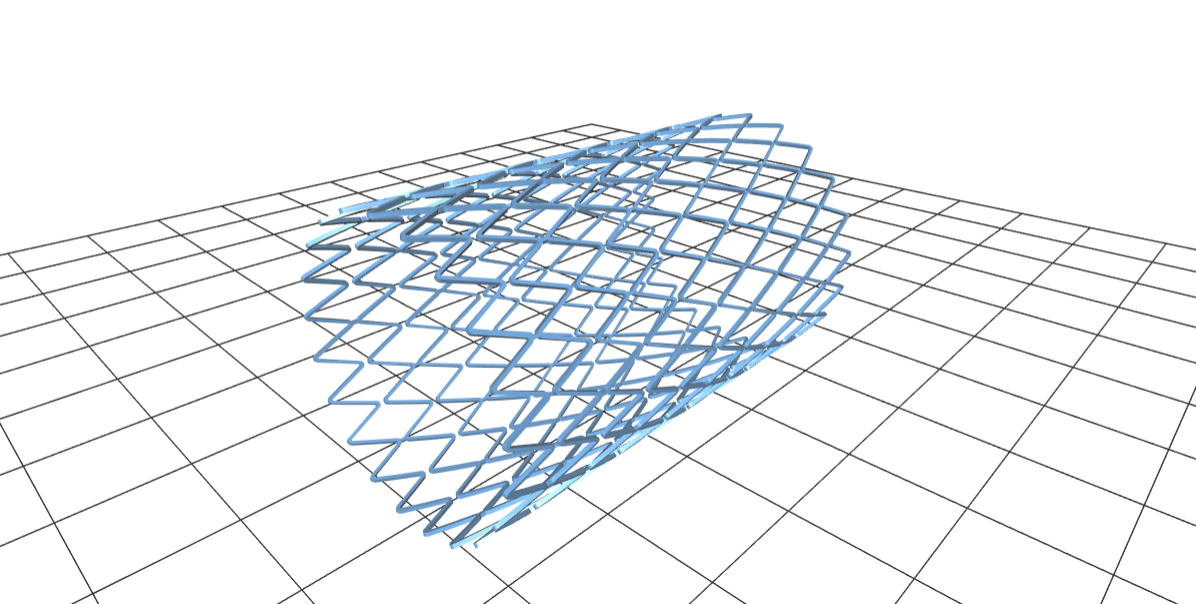
\includegraphics[width=3.5in]{Stent.PNG}
  \caption{An open stent design in the expanded state}
  \label{fig:stent}
\end{figure}
%
\vspace{7pt}
\section{Methodology}
%
We simulate a three dimensional model of a magnesium cardiovascular stent and monitor the corrosion through the millimeter electromagnetic backscattering. The simulations were carried out using the frequency domain solver of CST Microwave Studio.  For a stent composed of a mesh of wires as shown in Fig. \ref{fig:stent}, the corrosion only affects the cross-sectional area of the wire and it is independent of the length of the structure \cite{bowen2015rates}. The corrosion rate $P$ of a wire with an initial radius $r_0$, at any given time $t$ is,
%
\begin{equation}
  P = \dv{r}{t} = \frac{r_0 - r(t)}{t}
  \label{eq:corrosion}
\end{equation}
%
where $r(t)$ is the wire radius at time $t$.
%
In this paper, we used the \emph{Open stents} CAD model which is fully customizable due to its inherent parameterization \cite{bonsignore_open_2012}. The stent length was set to \SI{25}{\mm} with the diameter in the expanded state equal to \SI{4}{\mm}. The stent strut thickness was initially set to \SI{.2}{\mm}. Using \eqref{eq:corrosion}, a penetration corrosion rate of \SI{1.94}{\mm \per \year} for a magnesium alloy (AZ31) \cite{YU2017330} would leave behind \SI{.125}{\mm} thick wire after a \num{2} weeks period, and considering $P$ as uniform, the structure will be completely absorbed after \num{6} weeks.
%
We simulated the scattering response by progressively decreasing the strut thickness of the stent. To reduce the computational cost, we assumed the background material as free space. A point dipole was used to create the excitation signal.
%
\begin{figure}[h!]
  \centering
  \includegraphics[width=.85\linewidth]{stent_scattering.tex}
  \caption{Backscattering for different strut thicknesses}
  \label{fig:bcs}
\end{figure}
%
%
%
\vspace{7pt}
\section{Results and Discussion}
%
Figure \ref{fig:bcs} shows the backscattering from the open stent model described earlier with varying thicknesses. Although it is well known that the resonant frequency of a dipole antenna is only dependent upon the length, however, the electromagnetics of meshed structures such as the stent is complex due to its partially transparent nature to the wave. Table \ref{tab:resonance} lists the resonant frequencies extracted from Fig. \ref{fig:bcs}, and interestingly, a linearly decreasing frequency shift is observed as the stent is progressively corroded.
%
\begin{table}[!h]
  \centering
  \renewcommand{\arraystretch}{1.3}
  \caption{Effect of thickness on the resonant frequency}
  \centering
  \begin{tabularx}{.65\columnwidth}{c c}
    \toprule
    Thickness (mm) & Resonant Frequency (GHz)\\
    \midrule \midrule
    \num{0.2} & \num{237.2} \\
    \num{0.075} & \num{230.2} \\
    \num{0.02} & \num{227} \\
    \bottomrule \\
  \end{tabularx}
  \label{tab:resonance}
\end{table}
%

\vspace{7pt}
\section{Conclusion}
%
In this paper, we presented a non-invasive technique to progressively monitor the degradation of a magnesium based bio-absorbable cardiovascular stent using millimeter waves.
The proposed frequency range can provide sufficient spatial resolution and penetration without applying any radiation damage to the tissue. The fast corrosion rate of magnesium based biomaterials points to great potentials in designing cardiovascular stents. However, question marks on the structural integrity and corrosion remnants have restricted their popularization. In this preliminary report, we addressed some of these concerns by proposing a corrosion monitoring scheme that can non-invasively track the structural degradation by observing the frequency shift in the electromagnetic scattering.
% conference papers do not normally have an appendix
% use section* for acknowledgement
\vspace{7pt}
\section*{Acknowledgment}
%
This publication was made possible by Sidra Internal Research Fund grant number SIRF 200041 from the
Sidra Medicine (a member of Qatar Foundation). The statements made herein are solely the responsibility of the authors.





% trigger a \newpage just before the given reference
% number - used to balance the columns on the last page
% adjust value as needed - may need to be readjusted if
% the document is modified later
%\IEEEtriggeratref{8}
% The "triggered" command can be changed if desired:
%\IEEEtriggercmd{\enlargethispage{-5in}}

% references section

% can use a bibliography generated by BibTeX as a .bbl file
% BibTeX documentation can be easily obtained at:
% http://www.ctan.org/tex-archive/biblio/bibtex/contrib/doc/
% The IEEEtran BibTeX style support page is at:
% http://www.michaelshell.org/tex/ieeetran/bibtex/
%\bibliographystyle{IEEEtran}
% argument is your BibTeX string definitions and bibliography database(s)
%\bibliography{IEEEabrv,../bib/paper}
%
% <OR> manually copy in the resultant .bbl file
% set second argument of \begin to the number of references
% (used to reserve space for the reference number labels box)
\vspace{7pt}


\bibliographystyle{IEEEtran}
% \bibliographystyle{ieeetr}
% \atColsEnd{\vfil}
% argument is your BibTeX string definitions and bibliography database(s)
\bibliography{References}


% that's all folks
\end{document}
